\titleformat
{\chapter} % command
[display] % shape
{\bfseries\Huge} % format
{ } % label
{2ex} % sep
{
    %\vspace{1ex}
} % before-code
[ \vspace{0ex}
] % after-code

\raggedbottom % Allow flexible page heights to reduce underfull vbox warnings

\chapter[Xpressor: Towards foundation models that learn across biological scales]{Xpressor: Towards foundation models that learn across biological scales}
\label{article2}

\section{Summary}
Biological foundation models now exist across four scales: molecules, sequences, cells, and tissues; yet, they operate in isolation. We present a general approach, called Xpressor, for multi-scale learning via (1) compression, using a cross-attention mechanism, and (2) fine-tuning of the compression model. Applied to a cell foundation model, our gene-to-cell compression approach improves cell-type prediction (+28\%) and embedding quality (+8\%). Our amino-acid-to-gene fine-tuning approach also yields improvements across all metrics. The Xpressor represents a first step towards models that bridge biological scales.

\section{Introduction}

While it could be said of most domains, biology is a great example of a system that processes information across scales, from molecules to tissues. Foundation models now excel at specific scales: e.g., protein structures \citep{esm2}, cell states \citep{scprint, cuiScGPTBuildingFoundation2024}, but operate in isolation, unable to leverage cross-scale connections.

Our premise is that lower-scale information (e.g., molecular) can improve higher-scale representations (e.g., cellular), and vice versa \citep{bunneHowBuildVirtual2024, songAIDrivenDigitalOrganism2024}. While learning across all scales simultaneously is infeasible, we propose to compose pre-trained ``uniscale'' models through architectural updates and fine-tuning (see Figure~\ref{fig:scales}).

\subsection{Bio-foundation models across scales}
\label{sec:foundation_models}
Bio-foundation models exist at four biological scales (see Supplementary Material~\ref{sec:foundation_models_detail} for an extended review):

\textbf{Molecular FMs (\glspl{mFM})} encode molecules via \gls{SMILES} or 3D coordinates to predict binding, solubility, and dynamics \citep{abramsonAccurateStructurePrediction2024, mendez-lucioMolEFoundationModel2024}.

\textbf{Nucleotide FMs (\glspl{nFM})} use transformer-based language models on \gls{DNA}, \gls{RNA}, and protein sequences \citep{esm2, dalla-torreNucleotideTransformerBuilding2024}. We include protein language models in this category, as their distinctions are blurring \citep{brixiGenomeModelingDesign2025}.

\textbf{Cell FMs (\glspl{cFM})} are trained on single-cell \gls{RNA-seq} abundance matrices using encoder transformers \citep{scprint, cuiScGPTBuildingFoundation2024, theodorisTransferLearningEnables2023}. Challenges remain around data noise and coverage \citep{bendidiBenchmarkingTranscriptomicsFoundation2024}.

\textbf{Tissue FMs (\glspl{tFM})} learn spatial cell relationships from microscopy using vision transformers \citep{oquabDINOv2LearningRobust2024, chief}. Their tokens could leverage cell representations from \gls{cFM}s.

\begin{figure}[h]
\begin{center}
\includegraphics[width=0.5\linewidth] {figures/xpressor/scales}
\end{center}
\caption{Biological scales and how foundation model representations at each scale can inform adjacent scales. In red, we apply our proposed Xpressor approach.}
\label{fig:scales}
\end{figure}

\subsection{Existing approaches}
\paragraph{Architectural modifications: compressed representations}
Prior work on biological representations includes \gls{VAE}s \citep{scvi, scarches} and quantized embeddings \citep{cheap, mentzerFiniteScalarQuantization2023}. Simple pooling of transformer outputs performs poorly \citep{leeNVEmbedImprovedTechniques2025, ilseAttentionbasedDeepMultiple2018}; state-of-the-art methods instead use cross-attention mechanisms. We adopt a similar approach to compress foundation model outputs into lower-dimensional vectors.

\paragraph{Training modifications: fine-tuning}
Fine-tuning approaches range from full model updates to parameter-efficient methods like \gls{LoRA} \citep{lora, qlora} and adapter layers \citep{efficientft}, small \gls{MLP}s in-between model layers or outputs, each offering a lightweight and parameter-efficient approach. We will use adapter layers as a simpler proxy to Xpressor for fine-tuning lower-scale models.

\subsection{Contributions}
Following up on these recent advances, we propose:

\begin{itemize}
   \item A cross-attention "compressor" block whose goal is to compress a foundation model's output embeddings into a small set of low-dimensional vectors, called the \emph{Xpressor} (Cross-Attention Compressor transformer). This is learnt using an auto-encoding approach with a reconstruction loss. The Xpressor is modality-agnostic and can be used by \gls{mFM}s, \gls{nFM}s, \gls{cFM}s, \gls{tFM}s, or any other transformer-based foundation model, unregarding of the  pre-training tasks (see Figure~\ref{fig:first}A).
   \item A multi-scale fine-tuning approach using Xpressor. This allows the fine-tuning of models from one level using the upper-scale model's task (see Figure~\ref{fig:first}B).
\end{itemize}

\section{Xpressor}

\subsection{Background}
We use \gls{scPRINT} \citep{scprint} as our \gls{cFM} and \gls{ESM}2 \citep{esm2} as our \gls{nFM}. Below, we detail \gls{scPRINT}'s architecture and training, which inform our design choices.

\begin{figure}[H]
\begin{center}
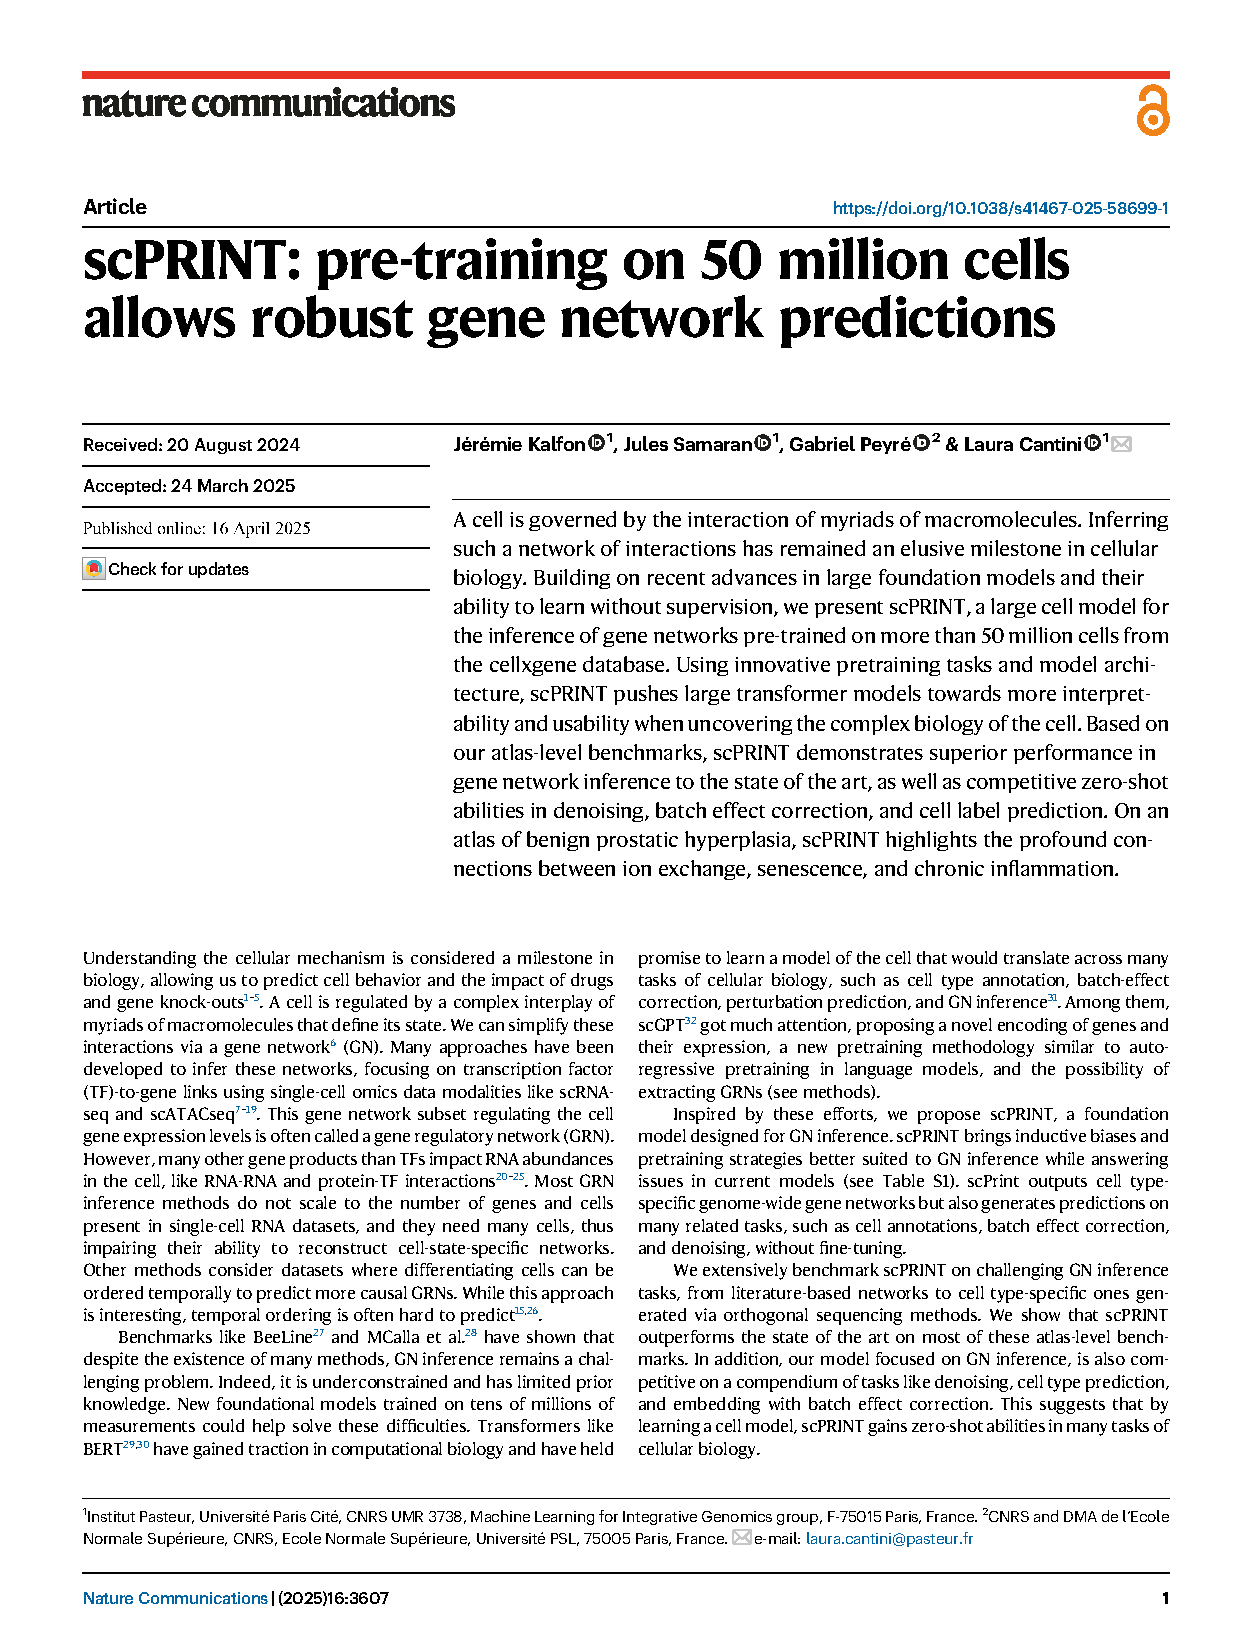
\includegraphics[width=0.9\linewidth]{figures/xpressor/scprint}
\end{center}
\caption{Overview of \gls{scPRINT}'s architecture: gene embeddings are formed by summing gene ID, expression, and positional embeddings. The transformer processes these along with cell and label tokens. The decoder outputs parameters of a zero-inflated negative binomial distribution for each gene. Inspired by the original Figure 1.A in \citet{scprint}.}
\label{fig:scprint}
\end{figure}

\textbf{Architecture.} \gls{scPRINT} is a bidirectional transformer trained on 50M+ cells from CellxGene \citep{programCZCELLxGENEDiscover2023}. Each gene in a cell is encoded as the sum of three embeddings: (1) a \emph{gene ID embedding} from \gls{ESM}2's mean-pooled amino acid embeddings of the gene's protein product, providing evolutionary and structural priors; (2) an \emph{expression embedding} from an \gls{MLP} applied to log-normalized counts $\mathbf{e}_{i,j} = \text{MLP}(\log_2(x_{i,j} + 1))$; and (3) a \emph{positional embedding} encoding genomic location, since co-located genes share regulatory regions. Additionally, learned placeholder tokens for cell embeddings and labels (cell type, disease, sex, etc.) are concatenated to form the input (see Figure~\ref{fig:scprint}).

The model processes 2,200 genes per cell during training (covering 80\% of cells in CellxGene), padding with unexpressed genes when needed. This lets the model distinguish true zeros from dropouts. The expression decoder outputs parameters of a zero-inflated negative binomial (\gls{ZINB}) distribution $(\mu, \theta, \pi)$ for each gene, modeling both the mean expression and overdispersion.

\textbf{Pretraining.} \gls{scPRINT} uses three jointly optimized tasks: (1) \emph{denoising}, reconstructing expression from downsampled profiles (60\% dropout), which encourages learning gene-gene interactions \citep{leoteRegulatoryNetworkbasedImputation2022}; (2) \emph{bottleneck learning}, compressing and reconstructing profiles through cell embeddings (see Figure~\ref{fig:scprint_1} in Supplementary Material~\ref{sec:scprint_detail}); and (3) \emph{label prediction}, classifying cell type, disease, and other annotations using a hierarchical classifier that handles ontology-structured labels of varying granularity.

\textbf{Gene networks.} \gls{scPRINT} extracts cell-specific gene networks from its attention matrices, similar to \gls{ESM}2's contact prediction. These networks can be subsetted to transcription factor-gene connections and benchmarked against ground-truth networks.

For protein representations, \gls{ESM}2 \citep{esm2} learns evolutionary constraints from amino acid sequences and enables structure prediction via ESMfold \citep{esmfold}.

\subsection{Approach}
Our first contribution is the compression of output embeddings of foundation models using a transformer block and a bottleneck-learning method (whose basic theory is presented in Supplementary Material~\ref{sec:tishbi}): we call it the Xpressor (see Figure~\ref{fig:first}A). Compression / decompression is the key mechanism for transferring representations across scales (see Supplementary Material~\ref{sec:foundation_models}). To do so, we introduce an additional set of transformer blocks called "Xpressor blocks". In the context of \gls{scPRINT}, these blocks represent cell features.

\begin{figure}[H]
\begin{center}
\includegraphics[width=0.9\linewidth] {figures/xpressor/first}
\end{center}
\caption{Overview of the Xpressor architecture and multi-scale fine-tuning approach applied to a cell foundation model. A. The Xpressor architecture, composed of M layers, shows how gene-level representations are compressed into cell-state vectors through cross-attention over the output embeddings of a transformer, composed of N layers. These compressed representations are then decompressed back using the same initial transformer model with cross-attention, given the initial gene-level tokens. B. Example of the multi-scale fine-tuning setup illustrating how the adapter layer enables joint training of gene-level representations that are then used by a \gls{cFM}. C. Detailed structure of the transformer and Xpressor blocks showing the cross-attention and self-attention sub-blocks. Blue blocks are our contributions. Shaded blocks indicate inputs and outputs.}
\label{fig:first}
\end{figure}

%% input
We keep scPRINT's input the same: we use a set of summed up gene expression and gene ID tokens. The first ones are generated using an \gls{MLP} for each gene expression value in cell $j$, and the others are generated from \gls{ESM}2's output embeddings for each gene, aggregated with mean-pooling. The newly proposed Xpressor block uses as input a set of learned latent tokens $\mT$. It then performs cross-attention between the last layer of the gene embeddings and the latent tokens (see Figure~\ref{fig:first}A). The goal is for the Xpressor blocks to be of smaller dimensions and context size than the main blocks, such that we end up with $\mC_j$, a set of $n$ tokens of dimension $d_t$ generated from the encoded gene expression and ID matrices $\mE_j$ and $\mG$. Where $\mG$ and $\mE_j$ are sets of $m$ tokens of size $d_c$ representing the IDs of the genes and their corresponding expression in cell $j$, respectively, where $d_c < d_t$ and $n << m$. In this context, for a cell $j$, \gls{scPRINT} does:

\begin{equation}
\mO_j=\mathrm{scPRINT}(\mE_j + \mG)
\label{eq:compression1}
\end{equation}

Where scPRINT implies N layers of transformer blocks performing self-attention (see figure~\ref{fig:scprint} for the transformer architecture). Xpressor is then applied on its output:

\begin{equation}
\mC_j = \mathrm{Xpressor}(\mO_j, \mT)
\label{eq:compression2}
\end{equation}

Where Xpressor implies M layers of transformer blocks performing cross-attention on the output embeddings $\mO_j$ and self attention on $\mT$, with $\mT$, the learned set of input cell tokens, and $\mC_j$ being the cell tokens associated with the input expression $\mE_j$.

Both scPRINT's and Xpressor's transformer blocks possess a cross-attention architecture (see Figure~\ref{fig:first}C) such that we can finally do:

\begin{equation}
\hat{\mE}_j = \mathrm{scPRINT}(\mC_j, \mG)
\label{eq:decompression}
\end{equation}

Where scPRINT this time performs cross-attention on the cell tokens $\mC_j$ and self-attention on the gene ID tokens $\mG$ to reconstruct the expression values $\hat{\mE}_j$.

textcolor{red}{In this example, the decompression is done with gene ID tokens as input only ($\mG$) (see Figure~\ref{fig:first}A). These tokens are expression independent} and thus do not depend on $j$. In the context of protein language models, for example, this would be replaced by positional tokens.

As shown in Figure~\ref{fig:first}A, the \emph{Transformer} blocks are applied twice: first as an encoder (self-attention only), then as a decoder alongside the \emph{Xpressor}. Unlike the original transformer \citep{vaswaniAttentionAllYou2023}, cross-attention is performed first. Related ideas appear in \citet{leeNVEmbedImprovedTechniques2025}, where a single cross-attention layer, together with prompting and fine-tuning, is used to compress the context of a large language model.

%% training
In the cell foundation model context, the goal of the \emph{Xpressor} is to perform compression of the gene id \& expression tokens into a set of cell tokens similar to the classical information bottleneck from \citet{tishbyInformationBottleneckMethoda} (see Supplementary Material~\ref{sec:tishbi}). And vice-versa, to decompress the cell tokens back into an expression profile. This, together with the scPRINT's denoising and classification tasks, compose our pre-training objective (see Supplementary Material~\ref{sec:pretraining}).

In our case, each embedding corresponds to a different cell component. At training time, we present multiple losses to both regularize it and ensure differences across them, similar to what can be done in \gls{VAE}s (see Supplementary Material~\ref{sec:otherlosses}).

\subsection{Results}
We show that such an instantiation of the transformer leads to better performance over the gymnasium of tasks available in the \gls{scPRINT} \gls{cFM}.

\begin{table}[t]
\caption{Comparison of cell embedding approaches}
\label{table1}
\begin{center}
\begin{tabular}{@{}l@{\hspace{4pt}}c@{\hspace{4pt}}c@{\hspace{4pt}}c@{}}
\toprule
\textbf{Model} & \begin{tabular}[c]{@{}c@{}}Cell Label\\Pred.\end{tabular} & \begin{tabular}[c]{@{}c@{}}Embed.\\Quality\end{tabular} & \begin{tabular}[c]{@{}c@{}}Gene-Net\\Infer.\end{tabular} \\
\midrule
Class-pooling & 0.56 & 0.49 & 3.8,1.5 \\
\textbf{Xpressor} & \textbf{0.72} & \textbf{0.53} & \textbf{4.1,1.7} \\
negative ctrl. & 0.00 & 0.37 & 1.0,1.0 \\
default methods & 0.5 & 0.44 & 3.5,2.2 \\
\bottomrule
\end{tabular}
\end{center}
\end{table}

Indeed, we now look at three specific tasks: cell-type prediction, embedding quality, and gene-network inference. The tasks are the same as presented in \citet{scprint}.

"Embedding quality" refers to the average \gls{scIB} \citep{lueckenBenchmarkingAtlaslevelData2022} score for batch correction and biological consistency of cell embeddings. In this context, \gls{scIB} assesses the quality of embeddings using measures of similarity, nearest neighbors, and clustering.

Cell-label predictions are generated using a classifier on top of the cell embeddings generated by each model. We follow the approach of \citet{scprint} here, which was recently presented with a different mechanism in \citet{wangHierarchicalInterpretationOutofDistribution2024}. This classification task allows us to see how one can steer the model's embeddings to represent meaningful biological features.

Finally, we display two different metrics for gene-network inference. The gene network inference benchmark aims to estimate the quality of the self-attention matrices by comparing them to a gene-gene ground-truth matrix. Here we use \gls{EPR}, an odds-ratio measure in which, e.g., a value of N means that the predictions are N times as likely to be correct as a random guess. One is the \gls{EPR} score on the genome-wide perturb-seq gene network from BenGRN \citep{scprint}, while the second is the average \gls{EPR} of multiple predicted gene networks across various cell types compared to BenGRN's omnipath ground-truth gene network \citep{tureiOmniPathGuidelinesGateway2016}.

In our comparison, the class-pooling  approach is used, similarly to other cell foundation models, like scPRINT \& scGPT \citep{cuiScGPTBuildingFoundation2024,scprint}, where a class token is added to the model's input and an additional loss is placed on it: $argmin_{C_j}(||E_j - \mC_j \mG_j^T||_2)$. Both models use the same latent dimensions, architectures, training paradigm, and number of input tokens for both genes and cells.

We see that the Xpressor outperforms the simpler class-pooling approach on embedding quality and cell-label prediction, while gene-network inference results remain roughly the same.

We have also added two baselines: a negative control using an untrained model, and a default method where, for each task, common unsupervised single-cell methods are used: \gls{PCA} for embedding quality, CellTypist \citep{dominguezcondeCrosstissueImmuneCell2022} for cell-label prediction, and GENIE3 \citep{genie3} for gene-network inference.

We will now see how we can further train -or fine-tune- these representations using information from the upper scale. While Xpressor layers with their small set of low-dimensional tokens are best suited for this task, we will focus on a commonly available foundation model without modifying its architecture.

\section{Multi-scale Fine-tuning}

\subsection{Background}
To merge foundation models, we need a way to connect the lower-scale models to the upper one. It had been proposed in \citet{rosenUniversalCellEmbeddings2023, scprint} to use protein language model-based representations, like those of \gls{ESM}2, as input tokens for the models. This decreases the number of parameters the model has to learn; it allows the model to work on genes unseen at training time; moreover, it lets the model use information it would not have gained otherwise, such as protein structure, homology, and mutations.

\subsection{Approach}
We propose going beyond simply reusing lower-scale models' representations and fine-tuning them during the pre-training of the upper-scale model. We would use a foundation model pretrained with Xpressor blocks and updating only the Xpressor blocks during fine-tuning to achieve high parameter efficiency.

However, this exercise would require us to pre-train and assess a second foundation model. We opt instead for a proxy to Xpressor: using an adapter layer (see Figure~\ref{fig:first}B) on top of a mean-pooling of \gls{ESM}2's output embeddings. This approach is strictly less expressive than Xpressor and serves as a lower bound on the performance gains from multi-scale fine-tuning. With the adapter layer, each output embedding matrices $\mS_k$ of a genetic sequence $k$ of length $N$ from \gls{ESM}2 is mapped to a point in space $\vi$ using a smooth \& trainable function $MLP()$, a 2-layer neural-network:

\begin{equation}
\vi_{k} = MLP(\frac{1}{N}\sum_{i=0}^{N}\vs_{k,i})
\label{eq:adapter}
\end{equation}

By using a neural-network, we allow for an interpolation of the initial lower-scale representation towards a representation containing features learned from the upper-scale data \citep{constantinescuApproximationInterpolationDeep2024}.
In our case, we use \gls{ESM}2 as the lower-scale model and scPRINT as the upper-scale model. The initial \gls{ESM}2 embedding is known to capture the protein's sequence, evolutionary similarity, and constraints.

Indeed, this is what allows this representation to replace the multiple sequence alignment (\gls{MSA}) step in ESMfold \citep{esmfold}. We posit that this initial embedding already contains the information necessary to understand some rules governing gene interactions (homology and similar evolutionary constraints). However, representations from \gls{ESM}2 differ significantly from those of single-cell foundation models. Our goal is to enrich these representations with knowledge gained from co-expression information across millions of cells.

\subsection{Results}
We show that a \gls{cFM} trained on the pooled embeddings of a pretrained \gls{nFM} performs better on most tasks from the \citet{scprint} gymnasium benchmark than one trained on learned representations (see Table~\ref{table2}). This is possible because we allow the model to start from a very rich representation instead of a random set of vectors, while still giving it the flexibility to incorporate additional knowledge. Each foundation model tested uses the same latent dimensions, architectures, training, and number of input tokens. We report performance at the last epoch; training is stopped after 20 epochs.

\begin{table}[t]
\caption{Comparison of input-gene embedding approaches}
\label{table2}
\begin{center}
\begin{tabular}{@{}l@{\hspace{4pt}}c@{\hspace{4pt}}c@{\hspace{4pt}}c@{}}
\toprule
\textbf{Model} & \begin{tabular}[c]{@{}c@{}}Cell Label\\Pred.\end{tabular} & \begin{tabular}[c]{@{}c@{}}Embed.\\Quality\end{tabular} & \begin{tabular}[c]{@{}c@{}}Gene-Net\\Infer.\end{tabular} \\
\midrule
Random init. & 0.62 & 0.48 & 4.5,1.0 \\
ESM2 frozen & 0.56 & 0.49 & 3.8,1.5 \\
\textbf{ESM2 fine-tuned} & \textbf{0.70} & \textbf{0.49} & \textbf{4.5,2.4} \\
\bottomrule
\end{tabular}
\end{center}
\end{table}

We also show the difference in cell embeddings obtained between the regular transformer and the Xpressor (see Figure~\ref{fig:second}). The dataset is a challenging mix of modalities with varying batch effects and levels of noise. Cell types are also quite similar, making the task more difficult. We can see that the Xpressor embeddings exhibit more structure and better resolve different cell types than a transformer with class-pooling.

\begin{figure}[H]
\begin{center}
\includegraphics[width=0.9\linewidth] {figures/xpressor/second}
\end{center}
\caption{Comparison of cell embeddings between the regular transformer with class-pooling (left), \gls{scIB}: 0.43, and the Xpressor (right), \gls{scIB}: 0.48. The Xpressor embeddings exhibit greater structure and better resolve different cell types.}
\label{fig:second}
\end{figure}

Using \gls{ESM}2's embeddings enables scPRINT to work on genes and sequences unseen at training time, learn from an unlimited number of species, and integrate DNA, RNA, and protein-level information, such as mutations and structural variants.

Finally, unlike other methods, this version does not require updating the original model and can be added to the new model. Moreover, with this approach, scPRINT still maintains the ability to work on genes and sequences unseen during training.

\subsection{Applications}
This multi-scale fine-tuning approach has applications in any context where one wants to compress a foundation model's representation. We have discussed examples in improving foundation model's biological representation of cells and proteins. We have shown how this can be used to create multi-scale model compositions.

In the context of cell foundation models, we included the Xpressor into a larger methodological development: scPRINT-2 \citep{kalfonScPRINT2NextgenerationCell2025}. In this same work, we investigate the biological relevance, applicability, and generalization abilities of scPRINT-2.

But this approach can also be used in other contexts. For example, one could use it in language models to compress context windows or in vision transformers to compress image patches of large images for use in other tasks.

\section*{Scope and Limitations}

While our framework applies in principle to all biological scales (\gls{mFM} $\rightarrow$ \gls{nFM} $\rightarrow$ \gls{cFM} $\rightarrow$ \gls{tFM}), we focused our empirical validation on the nFM-to-cFM connection (ESM2 to \gls{scPRINT}). Extending this work to other scale transitions would require substantial effort across multiple dimensions:

\textbf{Implementation and expertise.} Each modality uses distinct architectures, data formats, and training paradigms. Molecular foundation models employ equivariant networks with 3D coordinate inputs; tissue models use vision transformers on multi-channel images. Reimplementing, updating, and retraining these models requires deep domain expertise in each field.

\textbf{Benchmarking infrastructure.} Comprehensive evaluation requires modality-specific benchmarks that capture biologically meaningful tasks. While scPRINT provides a gymnasium of tasks for cFMs, equivalent benchmarks for cross-scale learning at other transitions (e.g., \gls{mFM}-to-\gls{nFM} or \gls{cFM}-to-\gls{tFM}) do not yet exist and would need to be developed.

\textbf{Computational resources.} Training foundation models at scale demands significant compute. Full retraining of models like \gls{ESM}2 or tissue foundation models to incorporate cross-scale objectives would multiply this cost.

Importantly, our approach offers two paths forward for other modalities:

\begin{enumerate}
   \item \textbf{Full retraining with multi-scale objectives}: Models like \gls{ESM}2 could be retrained from scratch, adding Xpressor blocks which will then be fine-tuned during the training of upper-scale models (e.g., cell FMs), enabling end-to-end cross-scale learning.
   \item \textbf{Post-hoc Xpressor addition}: Xpressor blocks can be added on top of \emph{pretrained} foundation models and trained for reconstruction without ever modifying the base model weights. This lightweight approach preserves the original model's capabilities while enabling compression and cross-scale transfer, and requires only a fraction of the original training compute.
\end{enumerate}

The second approach is particularly promising for rapid adoption, as it allows practitioners to leverage existing pretrained models (ESM2, Nucleotide Transformer, DINO-based tissue models) without fully retraining them, adding only the Xpressor compression layer and fine-tuning on cross-scale objectives.

\section*{Conclusion}

We proposed a framework for compositional hierarchical foundation models across biological scales. Rather than training end-to-end, we compose models that distill key information for adjacent scales, enabling a shared vocabulary for biological entities across molecules, cells, and tissues.

We have presented one small piece in this approach, in which a cell foundation model (scPRINT) leverages and fine-tunes a protein sequence foundation model (\gls{ESM}2). We have also shown how Xpressor can compress the output representations of transformers into a small set of lower-dimensional vectors, bridging proteins to cells. Such an approach could be used to bridge molecules to proteins and cells to tissues by using compressed representations that are then fine-tuned. This is a promising backbone architecture for a general model going from atoms to tissues.

Future work should focus on using Xpressor's representations to power upper-scale models or the ability to learn a Xpressor on top of a pre-trained foundation model. The Xpressor approach could also be extended to decoder-based language models. Finally, fine-tuning using an adapter layer suffers from a major drawback: the non-additivity of \gls{MLP}s, and therefore the limited use of such fine-tuned models in other contexts beyond their compressed representations. Implementing intelligent \gls{GPU} scheduling and using \gls{LoRA}-like methods to fine-tune only Xpressor blocks will allow for more complex fine-tuning in \gls{GPU}-rich settings. We will need to show that this approach can be applied to other scales of biological representation and to generate benchmarks that better capture the diversity of real-world biological tasks across these scales.

\section*{Supplementary}

\subsection{Extended review of foundation models across scales}
\label{sec:foundation_models_detail}
\textbf{Molecular foundation models (mFM)} model molecules with atomistic precision using \gls{SMILES} notation or 3D coordinates \citep{abramsonAccurateStructurePrediction2024, mendez-lucioMolEFoundationModel2024, rossLargescaleChemicalLanguage2022}. They incorporate symmetry invariances \citep{batznerE3equivariantGraphNeural2022} and can predict binding affinities, solubility, and dynamics, though matching precise molecular dynamics methods remains challenging \citep{benali2025pushingaccuracylimitfoundation, rhodes2025orbv3atomisticsimulationscale}.

\textbf{Nucleotide foundation models (nFM)} analyze \gls{DNA}, \gls{RNA}, and protein sequences using transformer architectures \citep{vaswaniAttentionAllYou2023, nguyen2023hyenadnalongrangegenomicsequence}. Protein language models like \gls{ESM}2 \citep{esm2} enable structure prediction, while \gls{DNA}/\gls{RNA} models focus on regulatory mechanisms \citep{dalla-torreNucleotideTransformerBuilding2024, wangMultipurposeRNALanguage2024, brixiGenomeModelingDesign2025}. These representations encode evolutionary constraints and can inform protein-protein interactions \citep{cornmanOMGDatasetOpen2024a}. Future \gls{nFM}s could use compressed \gls{mFM} representations as tokens, enabling unified modeling of nucleotides and their modifications \citep{xiaNatureLMDecipheringLanguage2025}.

\textbf{Cell foundation models (cFM)} are trained on single-cell RNA-seq abundance matrices \citep{bunneHowBuildVirtual2024, scprint, theodorisTransferLearningEnables2023, cuiScGPTBuildingFoundation2024, haoLargescaleFoundationModel2024, rosenUniversalCellEmbeddings2023}. Despite promising benchmarks, experimental validations remain challenging due to data noise, limited coverage, and species bias \citep{bendidiBenchmarkingTranscriptomicsFoundation2024, boiarskyDeepDiveSingleCell2023, programCZCELLxGENEDiscover2023}. Distilling sequence-level knowledge onto cFMs could improve learning of regulatory mechanisms.

\textbf{Tissue foundation models (tFM)} learn spatial cell relationships from microscopy using vision transformers \citep{oquabDINOv2LearningRobust2024, chief, brayCellPaintingHighcontent2016, wencksternAIpoweredVirtualTissues2025}. Spatial transcriptomics modalities provide rich channel information but at limited resolution \citep{alonExpansionSequencingSpatially2021}. Challenges include data accessibility, 2D limitations, and measuring cell communication \citep{hertleHorizontalGenomeTransfer2021}. tFMs could use \gls{cFM} cell representations as tokens to predict cell presence in spatial context.

\subsection{Detailed scPRINT architecture and training}
\label{sec:scprint_detail}

We provide here additional details on scPRINT's architecture and training procedure, which serve as the foundation for our Xpressor contributions.

\subsubsection{Expression encoder}
Each gene $j$ in cell $i$ is represented as the sum of three embeddings:
\begin{equation}
\mathbf{x}_{i,j} = \mathbf{g}_j + \mathbf{e}_{i,j} + \mathbf{l}_j
\end{equation}
where $\mathbf{g}_j \in \mathbb{R}^d$ is the gene identity embedding, $\mathbf{e}_{i,j} \in \mathbb{R}^d$ is the expression embedding, and $\mathbf{l}_j \in \mathbb{R}^d$ is the genomic location embedding.

\textbf{Gene identity embedding.} The gene embedding $\mathbf{g}_j$ is derived from \gls{ESM}2 by mean-pooling over all amino acid embeddings of the gene's canonical protein product. This provides evolutionary and structural priors while enabling generalization to unseen genes.

\textbf{Expression embedding.} The expression value is encoded via a two-layer \gls{MLP}:
\begin{equation}
\mathbf{e}_{i,j} = \text{MLP}(\log_2(x_{i,j} + 1)), \quad x_{i,j} \in \mathbb{R}_{\geq 0}
\end{equation}
where each \gls{MLP} layer applies: $\text{Dropout}(\text{ReLU}(\text{LayerNorm}(\text{Linear}(\cdot))))$ with dropout rate 0.1. This lets the model learn an appropriate metric for expression values, unlike binning (\gls{scGPT}) or ranking (Geneformer) approaches that impose specific priors.

\textbf{Genomic location embedding.} Genes within 10kb are assigned the same location index, then encoded using sinusoidal positional encoding \citep{vaswaniAttentionAllYou2023}. This captures the fact that co-located genes often share regulatory regions.

The full input to the transformer for cell $i$ is:
\begin{equation}
X_i = [\mathbf{x}_{i,1}, \ldots, \mathbf{x}_{i,m}, \mathbf{e}_{t,i}, \mathbf{p}_{\text{cell}}, \mathbf{p}_{\text{type}}, \mathbf{p}_{\text{disease}}, \ldots]
\end{equation}
where $\mathbf{e}_{t,i} = \text{MLP}(\log_2(1 + t_i))$ encodes the total count $t_i = \sum_j x_{i,j}$, and $\mathbf{p}_{\cdot}$ are learned placeholder tokens for cell embeddings and label predictions.

\subsubsection{Transformer architecture}
\gls{scPRINT} uses a bidirectional transformer with $n$ layers, $h$ attention heads, and dimension $d$. Key implementation choices include:
\begin{itemize}
   \item FlashAttention2 for efficient attention computation
   \item Pre-normalization with fused LayerNorm
   \item Stochastic depth with linearly increasing dropout (0.02 per layer)
   \item 2-layer MLP with 4$\times$ hidden dimension and GELU activation
\end{itemize}

During training, 2,200 genes are sampled per cell (covering $>$80\% of CellxGene cells). When fewer genes are expressed, the input is padded with randomly sampled unexpressed genes, allowing the model to distinguish true zeros from dropouts.

\subsubsection{Expression decoder}
The decoder outputs parameters of a zero-inflated negative binomial (\gls{ZINB}) distribution for each gene:
\begin{equation}
\mu_j, \theta_j, \pi_j = \text{MLP}(\mathbf{o}_j)
\end{equation}
where $\mathbf{o}_j$ is the transformer output for gene $j$. The ZINB distribution is defined as:
\begin{equation}
\text{ZINB}(x \mid \mu, \theta, \pi) = \pi \cdot \delta_0(x) + (1 - \pi) \cdot \text{NB}(x \mid \mu, \theta)
\end{equation}
where $\delta_0(x)$ is a point mass at zero, and the negative binomial is:
\begin{equation}
\text{NB}(x \mid \mu, \theta) = \frac{\Gamma(x + \theta)}{x! \, \Gamma(\theta)} \left(\frac{\mu}{\mu + \theta}\right)^x \left(\frac{\theta}{\mu + \theta}\right)^\theta
\end{equation}
Here $\mu$ is the mean and $\theta$ is the inverse dispersion. Unlike \gls{scVI}, which learns a fixed $\theta$ per gene, \gls{scPRINT} predicts it dynamically, allowing the model to capture context-dependent overdispersion.

\subsubsection{Pretraining objectives}
\label{sec:pretraining}
\begin{figure}[H]
\begin{center}
\includegraphics[width=0.8\linewidth]{figures/xpressor/scprint_1}
\end{center}
\caption{Overview of scPRINT's pretraining tasks. Three pretraining objectives are jointly optimized: denoising (reconstructing from downsampled profiles), bottleneck learning (compression through cell embeddings), and label prediction (hierarchical classification of cell annotations). Inspired by the original Figure 1.B in \citet{scprint}.}
\label{fig:scprint_1}
\end{figure}

The total loss is: $\mathcal{L} = \mathcal{L}_{\text{denoise}} + \mathcal{L}_{\text{bottleneck}} + \mathcal{L}_{\text{classify}}$

\textbf{Denoising loss.} Expression profiles are downsampled using a zero-inflated Poisson model with dropout rate $r = 0.6$:
\begin{equation}
\tilde{x}_{i,j} \sim \text{ZiPoisson}(x_{i,j}, r)
\end{equation}
The model reconstructs the original counts, with loss given by the negative log-likelihood under the \gls{ZINB} decoder (see Figure~\ref{fig:scprint_1}).

\textbf{Bottleneck loss.} The model must reconstruct expression from cell embeddings alone (without gene expression inputs), encouraging compression of cellular state into the placeholder tokens (see Figure~\ref{fig:scprint_1}).

\textbf{Classification loss.} For hierarchical labels (cell type, disease, assay), we use a modified cross-entropy that handles ontology structure. For non-leaf labels, we apply log-sum-exp over descendant leaf labels:
\begin{equation}
\mathcal{L}_{\text{cls}} = \text{CE}(\bar{\mathbf{c}}, \mathbf{c}), \quad \bar{c}_k = \begin{cases} \hat{c}_k & \text{if } k \in \mathcal{T} \\ \text{LSE}(\{\hat{c}_l : l \in \text{desc}(k)\}) & \text{otherwise} \end{cases}
\end{equation}
where $\mathcal{T}$ is the set of leaf labels and $\text{desc}(k)$ are descendants of label $k$ (see Figure~\ref{fig:scprint_1}).

\subsubsection{Optimization}
Training uses fused AdamW with weight decay 0.01, learning rate $10^{-4}$, and stochastic weight averaging (SWA) with LR 0.03. Sub-epochs consist of 7,000 training and 2,000 validation batches with a 500-step warmup. Learning rate decays by 0.6$\times$ with patience 1, and training stops after 3 consecutive validation loss increases. Weighted random sampling with factor 50 balances rare cell types: sampling weight $\propto \frac{50}{\text{count} + 50}$.

\subsubsection{Gene network extraction}
Cell-specific gene networks are extracted from attention matrices, following \gls{ESM}2's approach for contact prediction. For a cell $i$, the gene-gene attention matrix $A_i \in \mathbb{R}^{m \times m}$ captures learned interactions. These can be thresholded to obtain sparse networks or subset to transcription factor-gene edges for gene regulatory network (\gls{GRN}) inference. Attention heads can be selected based on correlation with ground-truth networks to focus on biologically meaningful interactions.

More details on \gls{scPRINT}'s pre-training and architecture, datasets preprocessing, and gene network extraction are available in \citet{scprint}.

\subsection{argument about the Tishby et al. bottleneck learning approach}
\label{sec:tishbi}
We present the Information Bottleneck (\gls{IB}) method, a technique that defines compression as a learning approach. Using the information theory framework, it seeks a stochastic mapping \( p(t|x) \) that compresses the input variable \( X \) into a representation \( T \), while preserving as much information as possible about the relevant variable \( Y \). The trade-off is controlled by the Lagrange multiplier \( \beta \geq 0 \). The \gls{IB} objective is to minimize the following Lagrangian:
\begin{equation}
\mathcal{L}_{\text{IB}}[p(t|x)] = I(X;T) - \beta\, I(T;Y),
\end{equation}
where \( I(\cdot;\cdot) \) denotes mutual information.

Under the Markov constraint
\(\mathbf{Y} \leftrightarrow \mathbf{X} \leftrightarrow \mathbf{T}\),
The optimization leads to the following self-consistent equations:
\begin{align}
p(t|x) &= \frac{p(t)}{Z(x,\beta)} \exp\left(-\beta\, D_{\mathrm{KL}}\bigl(p(y|x) \,\|\, p(y|t)\bigr)\right), \label{eq:ib_ptx} \\
p(t) &= \sum_{x} p(x)\, p(t|x), \label{eq:ib_pt} \\
p(y|t) &= \frac{1}{p(t)} \sum_{x} p(y|x)\, p(x)\, p(t|x), \label{eq:ib_pyt}
\end{align}
where:
\begin{itemize}
   \item \( D_{\mathrm{KL}}\bigl(p(y|x) \,\|\, p(y|t)\bigr) \) is the Kullback-Leibler divergence between the conditional distributions \( p(y|x) \) and \( p(y|t) \),
   \item \( Z(x,\beta) \) is the normalization factor ensuring that \( \sum_t p(t|x) = 1 \).
\end{itemize}

\subsection{FSQ and other contrastive losses on the cell embeddings}
\label{sec:otherlosses}
While \(D_{\mathrm{KL}}\) over a non-informative Gaussian prior is a common formulation for regularizing the embedding space in \gls{VAE}s, other formulations have been used, such as with the \gls{VQ-VAE} and \gls{FSQ-VAE}. In these contexts, the \(D_{\mathrm{KL}}\) is replaced with a discretization objective tailored to the respective quantization schemes.

\paragraph{VQ-VAE.}
Value Quantized (VQ)-VAE employs a \emph{codebook} of size \(C\), where each codebook entry is a \(d\)-dimensional vector. The encoder produces a continuous latent vector, which is then mapped to its nearest codebook entry (a hard quantization). A commitment loss term encourages the encoder's outputs to stay close to the chosen codebook vector, making the entire latent representation discrete at the vector level.

\paragraph{FSQ-VAE.}
By contrast, Finite Scalar Quantization (FSQ)-VAE discretizes each latent dimension \emph{independently}. Specifically, the encoder outputs \(d\) values, each constrained to lie within a bounded range (e.g., \([-1, 1]\)). Each dimension is then quantized into one of \(M\) discrete levels within that range. This dimension-wise quantization can be implemented as either a hard nearest-bin assignment or a differentiable approximation thereof. Because \gls{FSQ} enforces scalar-level discretization, it provides a simpler and more fine-grained alternative to VQ's vector-level codebook approach, while still offering strong regularization of the latent space.

\paragraph{Contrastive regularization across embedding dimensions.}
We further encourage each of the \(d\) embedding dimensions to encode distinct information by adding a contrastive loss between them. Specifically, we compute pairwise similarities among embedding elements and penalize redundancy, thus pushing each dimension to capture complementary features. A general contrastive loss for this purpose can be written as
\begin{equation}
\mathcal{L}_{\text{contrastive}} = \sum_{i=1}^{d} \sum_{j \neq i} \ell\bigl(\mathbf{e}_i, \mathbf{e}_j\bigr),
\label{eq:contrastive}
\end{equation}
where \(\mathbf{e}_i\) denotes the \(i\)-th embedding dimension and \(\ell\) is a contrastive loss function (e.g., InfoNCE \citep{oordRepresentationLearningContrastive2019}) that encourages \emph{dissimilarity} among different embedding components.

\paragraph{Dimension-specific classifiers.}
To further steer each dimension's content, one can add a separate classifier on top of each dimension to learn about different classes. The classifier for dimension \(i\) is trained via a cross-entropy loss
\begin{equation}
\mathcal{L}_{\text{cls}}^{(i)} = - \sum_{c} y_{c} \log p\bigl(c \mid \mathbf{e}_i\bigr),
\label{eq:cls_loss_i}
\end{equation}
where \(y_c\) is the ground-truth label and \(p\bigl(c \mid \mathbf{e}_i\bigr)\) is the predicted probability for class \(c\). Summing these per-dimension losses yields an overall classification objective
\begin{equation}
\mathcal{L}_{\text{cls}} = \sum_{i=1}^{d} \mathcal{L}_{\text{cls}}^{(i)}.
\label{eq:cls_loss_total}
\end{equation}
Together, the contrastive and classification losses ensure each embedding dimension captures unique, discriminative information, resulting in more expressive representations.


\section*{Software and Data}

The software and data for training scPRINT, as well as gymnasium tasks and code to reproduce the results of the manuscript, are available at \url{https://github.com/cantinilab/Xpressor}.

WandB logs are available in the following link:
\url{https://api.wandb.ai/links/ml4ig/h370j6io}

Model checkpoints are available at the following link:
\url{https://huggingface.co/jkobject/scPRINT/tree/main}



\section*{Acknowledgments}

The project leading to this manuscript has received funding from the Inception program (Investissement d'Avenir grant ANR-16-CONV-0005) L.C. and the European Union (ERC StG, MULTIview-CELL, 101115618) L.C. We acknowledge the help of the HPC Core Facility of the Institut Pasteur and Déborah Philipps for the administrative support. L.C.

The work of G. Peyré was supported by the French government under management of Agence Nationale de la Recherche as part of the 'Investissements d'avenir' program, reference ANR19-P3IA-0001 (PRAIRIE 3IA Institute). G.P.

\section*{Impact Statement}

This paper presents work aimed at advancing the fields of computational biology and machine learning. No ethical issues are raised by the work other than what is typically noted in computational biology and foundation model papers. It might have an impact on building better models for drug discovery, target discovery, and improving our understanding of biological systems.
